\documentclass{report}
\title{Congruency Theorems}
\author{Paul Roberts}
\date{}
\pagenumbering{gobble}
\usepackage{graphicx}
\usepackage{wrapfig}



\begin{document}

\chapter{Congruency Theorems in Neutral Geometry}

\textbf{Note on notation:} For a vertex $A$ in $\triangle{ABC}$, we may refer to the interior angle $\angle CAB$ as $\angle a$. We denote the length of a segment $\overline{\rm AB}$ as $|\overline{\rm AB}|$. We do not rely on any definition of length except to say that $|\overline{\rm AB}| = |\overline{\rm CD}| \iff \overline{\rm AB} \cong \overline{\rm CD}$. Everywhere a statement about equality of lengths is made, it is equivalent to a statement about congruence of line segments or radii of circles, but we have chosen this notation for clarity and consistency with modern geometry. We assume here that angles have a measurement such that they can be related in equality and added. In particular, we assume the cancellation law for measurements of angles under addition, namely $\angle a + \angle b = \angle a + \angle c \iff \angle b = \angle c$.
\\[\baselineskip]Theorems are indexed $X.Y$ and constructions are indexed $X.Y.Z$.


\section{Side-Angle-Side Congruence}
Two triangles are congruent if two sides and the included angle of one are congruent respectively to two sides and the included angle of the other.
\\[\baselineskip] \textit{Proof.} Let $\triangle{ABC}$ and $\triangle{A'B'C'}$ be constructed st. $\overline{\rm AB} \cong \overline{\rm A'B'}$, $\overline{\rm BC} \cong \overline{\rm B'C'}$, and $\angle b  \cong \angle b'$. Move $\triangle{A'B'C'}$ so that $\overline{\rm A'B'}$ coincides with $\overline{\rm AB}$, and so that $C$ and $C'$ are on the same side of $\overline{\rm AB}$. By the definition of congruent angles, $\overline{\rm BC}$ and $\overline{\rm B'C'}$, starting from the same point $B$ and extending out along $\angle b$ and $\angle b'$ respectively, coincide with each other. Since $\overline{\rm BC} \cong \overline{\rm B'C'}$, we know they have a common endpoint at $C$. Then, $\overline{\rm AC}$ and $\overline{\rm A'C'}$ are line segments connecting coinciding points $A, A'$ to coinciding points $C, C'$, so they must also coincide. Since we have now that each of the segments in $\triangle{ABC}$ coincides with a segment in $\triangle{A'B'C'}$, the two triangles are congruent.

\section{Angle-Side-Angle Congruence}
Two triangles are congruent if two angles and the included side of one are congruent respectively to two angles and the included side of the other.
\\[\baselineskip] \textit{Proof.} Let $\triangle{ABC}$ and $\triangle{A'B'C'}$ be constructed st. $\angle a \cong \angle a'$, $\overline{\rm AB} \cong \overline{\rm A'B'}$, and $\angle b \cong \angle b'$. Move $\triangle{A'B'C'}$ so that $\overline{\rm A'B'}$ coincides with $\overline{\rm AB}$, and so that $C$ and $C'$ are on the same side of $\overline{\rm AB}$. By the definition of congruent angles, $\overline{\rm BC}$ and $\overline{\rm B'C'}$, starting from the same point $B$ and extending out along $\angle b$ and $\angle b'$ respectively, coincide with each other. Similarly, by the definition of congruent angles, $\overline{\rm AC}$ and $\overline{\rm A'C'}$, starting from the same point $A$ and extending out along $\angle a$ and $\angle a'$ respectively, coincide with each other. By the definition of triangle, we know that $\overline{\rm AC}$ and $\overline{\rm BC}$ intersect at point $C$. Since $\overline{\rm A'C'}$ and $\overline{\rm B'C'}$ coincide with $\overline{\rm AC}$,$\overline{\rm BC}$ respectively, they must intersect at the point $C'$ which coincides with $C$. Since $A, B, C$ all coincide with $A', B', C'$, the two triangles are congruent.
\subsection{Construction of an Equilateral Triangle}
\begin{wrapfigure}{r}{0.35\textwidth} %this figure is placed at the right
    \centering
    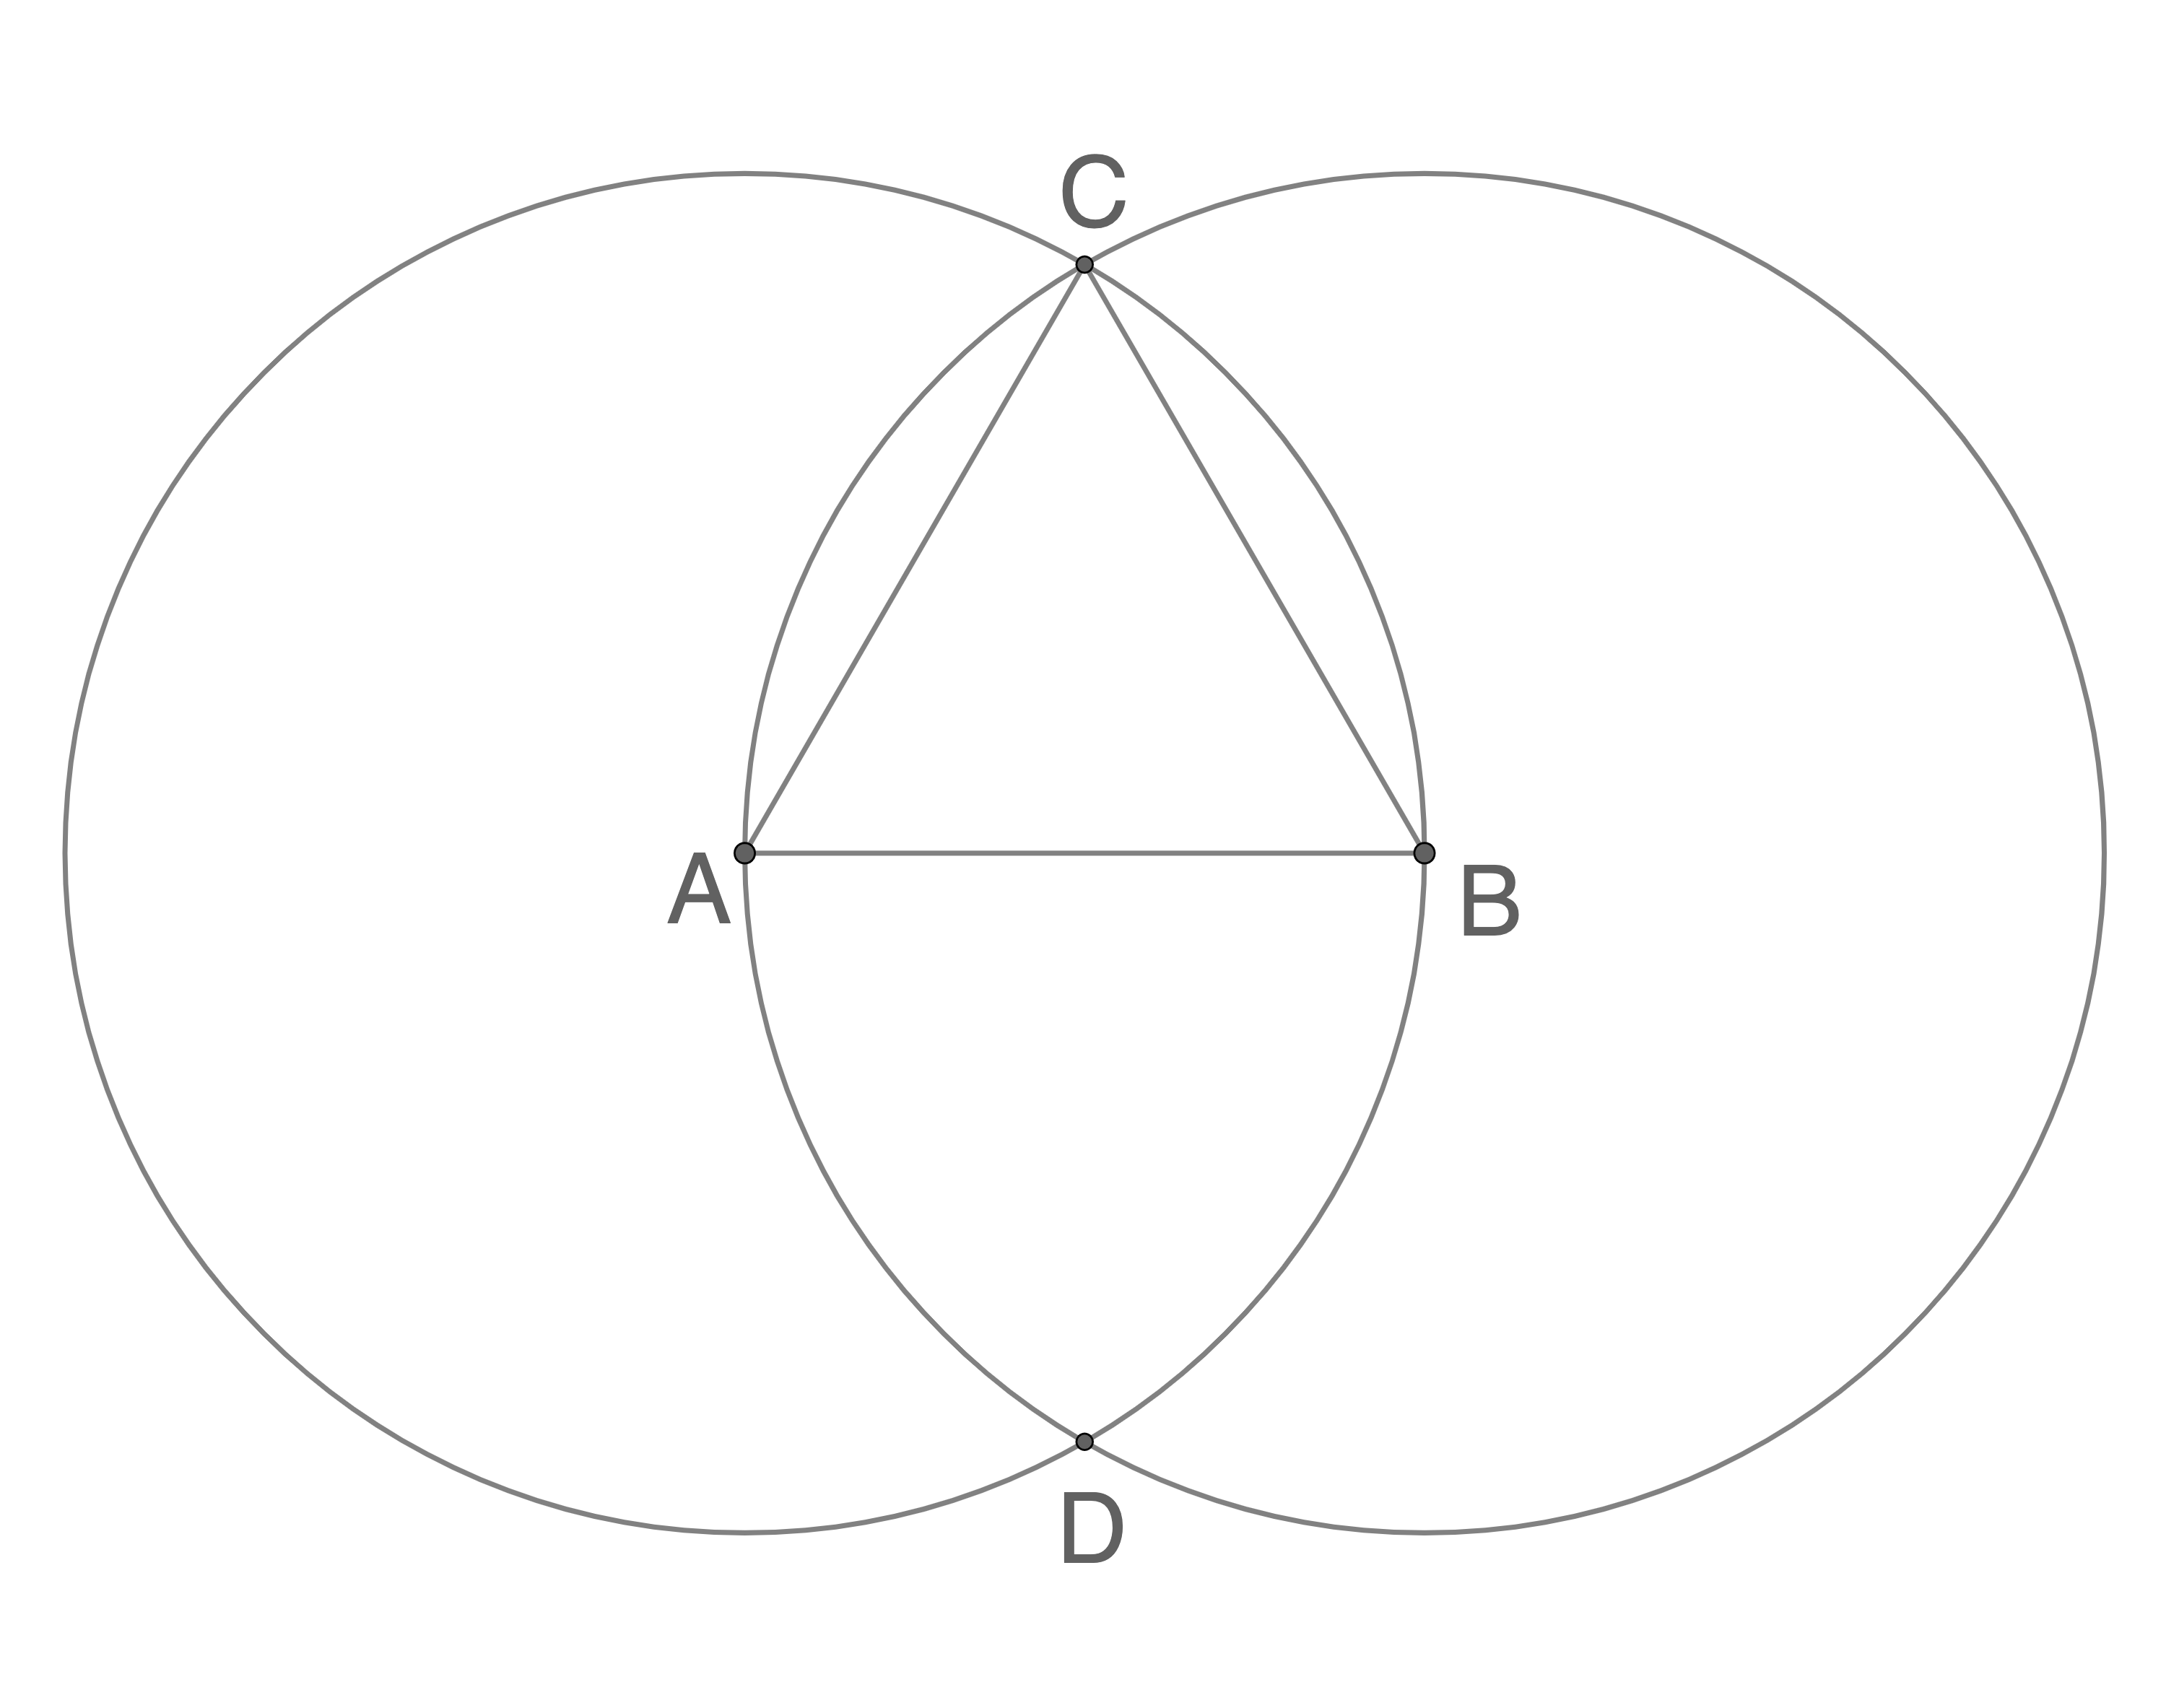
\includegraphics[width=0.35\textwidth]{eqtri}
\end{wrapfigure}
We will construct a triangle with three equal sides on a given base $\overline{\rm AB}$.
\\[\baselineskip]
Draw a circle $\alpha$ with radius $|\overline{\rm AB}|$ centered at $A$, and a circle $\beta$ with radius $|\overline{\rm BA}|$ centered at $B$ [Euclid Post.\@ 3]. Label a point of intersection of these circles $C$. Then $\triangle{ABC}$ is equilateral, since all points on $\alpha$, including $C$, have distance $|\overline{\rm AB}|$ from $A$, so $|\overline{\rm AC}|= |\overline{\rm AB}|$. We can conclude with an identical argument $|\overline{\rm BC}|= |\overline{\rm AB}|$, thus showing $\triangle{ABC}$ is equilateral.
\\Note that this method of construction allows for two different equilateral triangles, depending on the choice of which intersection of $\alpha$ and $\beta$ to use.
\subsection{Construction of a Given Length}
\begin{wrapfigure}{r}{0.35\textwidth} %this figure is placed at the right
    \centering
    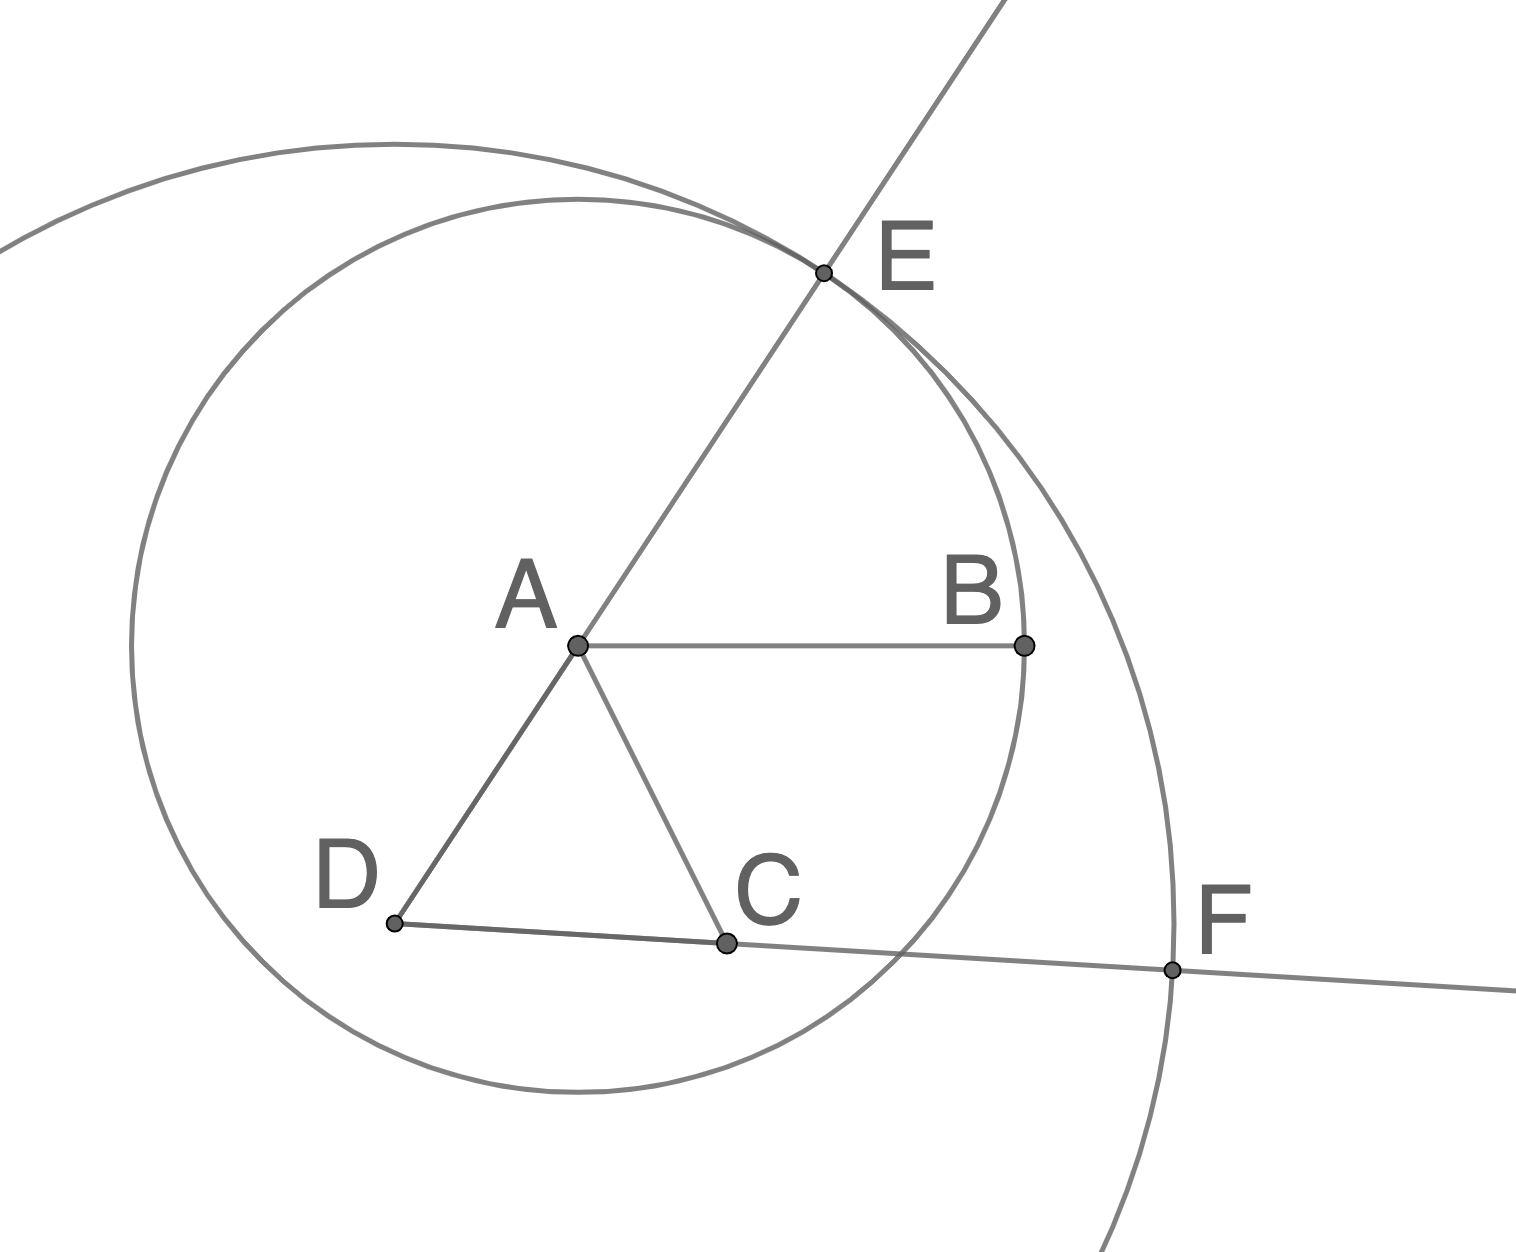
\includegraphics[width=0.35\textwidth]{fav}
\end{wrapfigure}
Given a line segment $\overline{\rm AB}$, and an arbitrary point $C$, we will construct a circle of radius $|\overline{\rm AB}|$ at $C$.
\\[\baselineskip]
Connect $A$ and $C$ with a line, and with base $\overline{\rm AC}$ construct the equilateral triangle $\triangle{ACD}$ (the choice of intersection for D does not matter). Draw a circle, $\alpha$, with a center at $A$ with a radius of $\overline{\rm AB}$. Continue the line segments $\overline{\rm DA}$ and $\overline{\rm DC}$ indefinitely. Label the point of intersection between the line $\overrightarrow{\rm DA}$ and $\alpha$ $E$. Then draw a circle, $\beta$ with center $D$ and radius $\overline{\rm DE}$. Label the intersection of $\overrightarrow{\rm DC}$ and $\beta$ $F$. Then, we claim $|\overline{\rm AE}| = |\overline{\rm CF}|$.
\\$|\overline{\rm DE}|=|\overline{\rm DF}|$, as they are both radii of $\beta$. We then have $|\overline{\rm DE}|=|\overline{\rm DA}|+|\overline{\rm AE}|=|\overline{\rm DC}|+|\overline{\rm CF}|=|\overline{\rm DF}|$. Since $|\overline{\rm DA}|=|\overline{\rm DC}|$, as they are both sides of the same equilateral triangle, we get $|\overline{\rm AE}| = |\overline{\rm CF}|$ from our former equality.
\subsection{Angle Bisection}
This will illustrate how to construct a line bisecting a given angle.
\\[\baselineskip]
\begin{wrapfigure}{r}{0.35\textwidth} %this figure is placed at the right
    \centering
    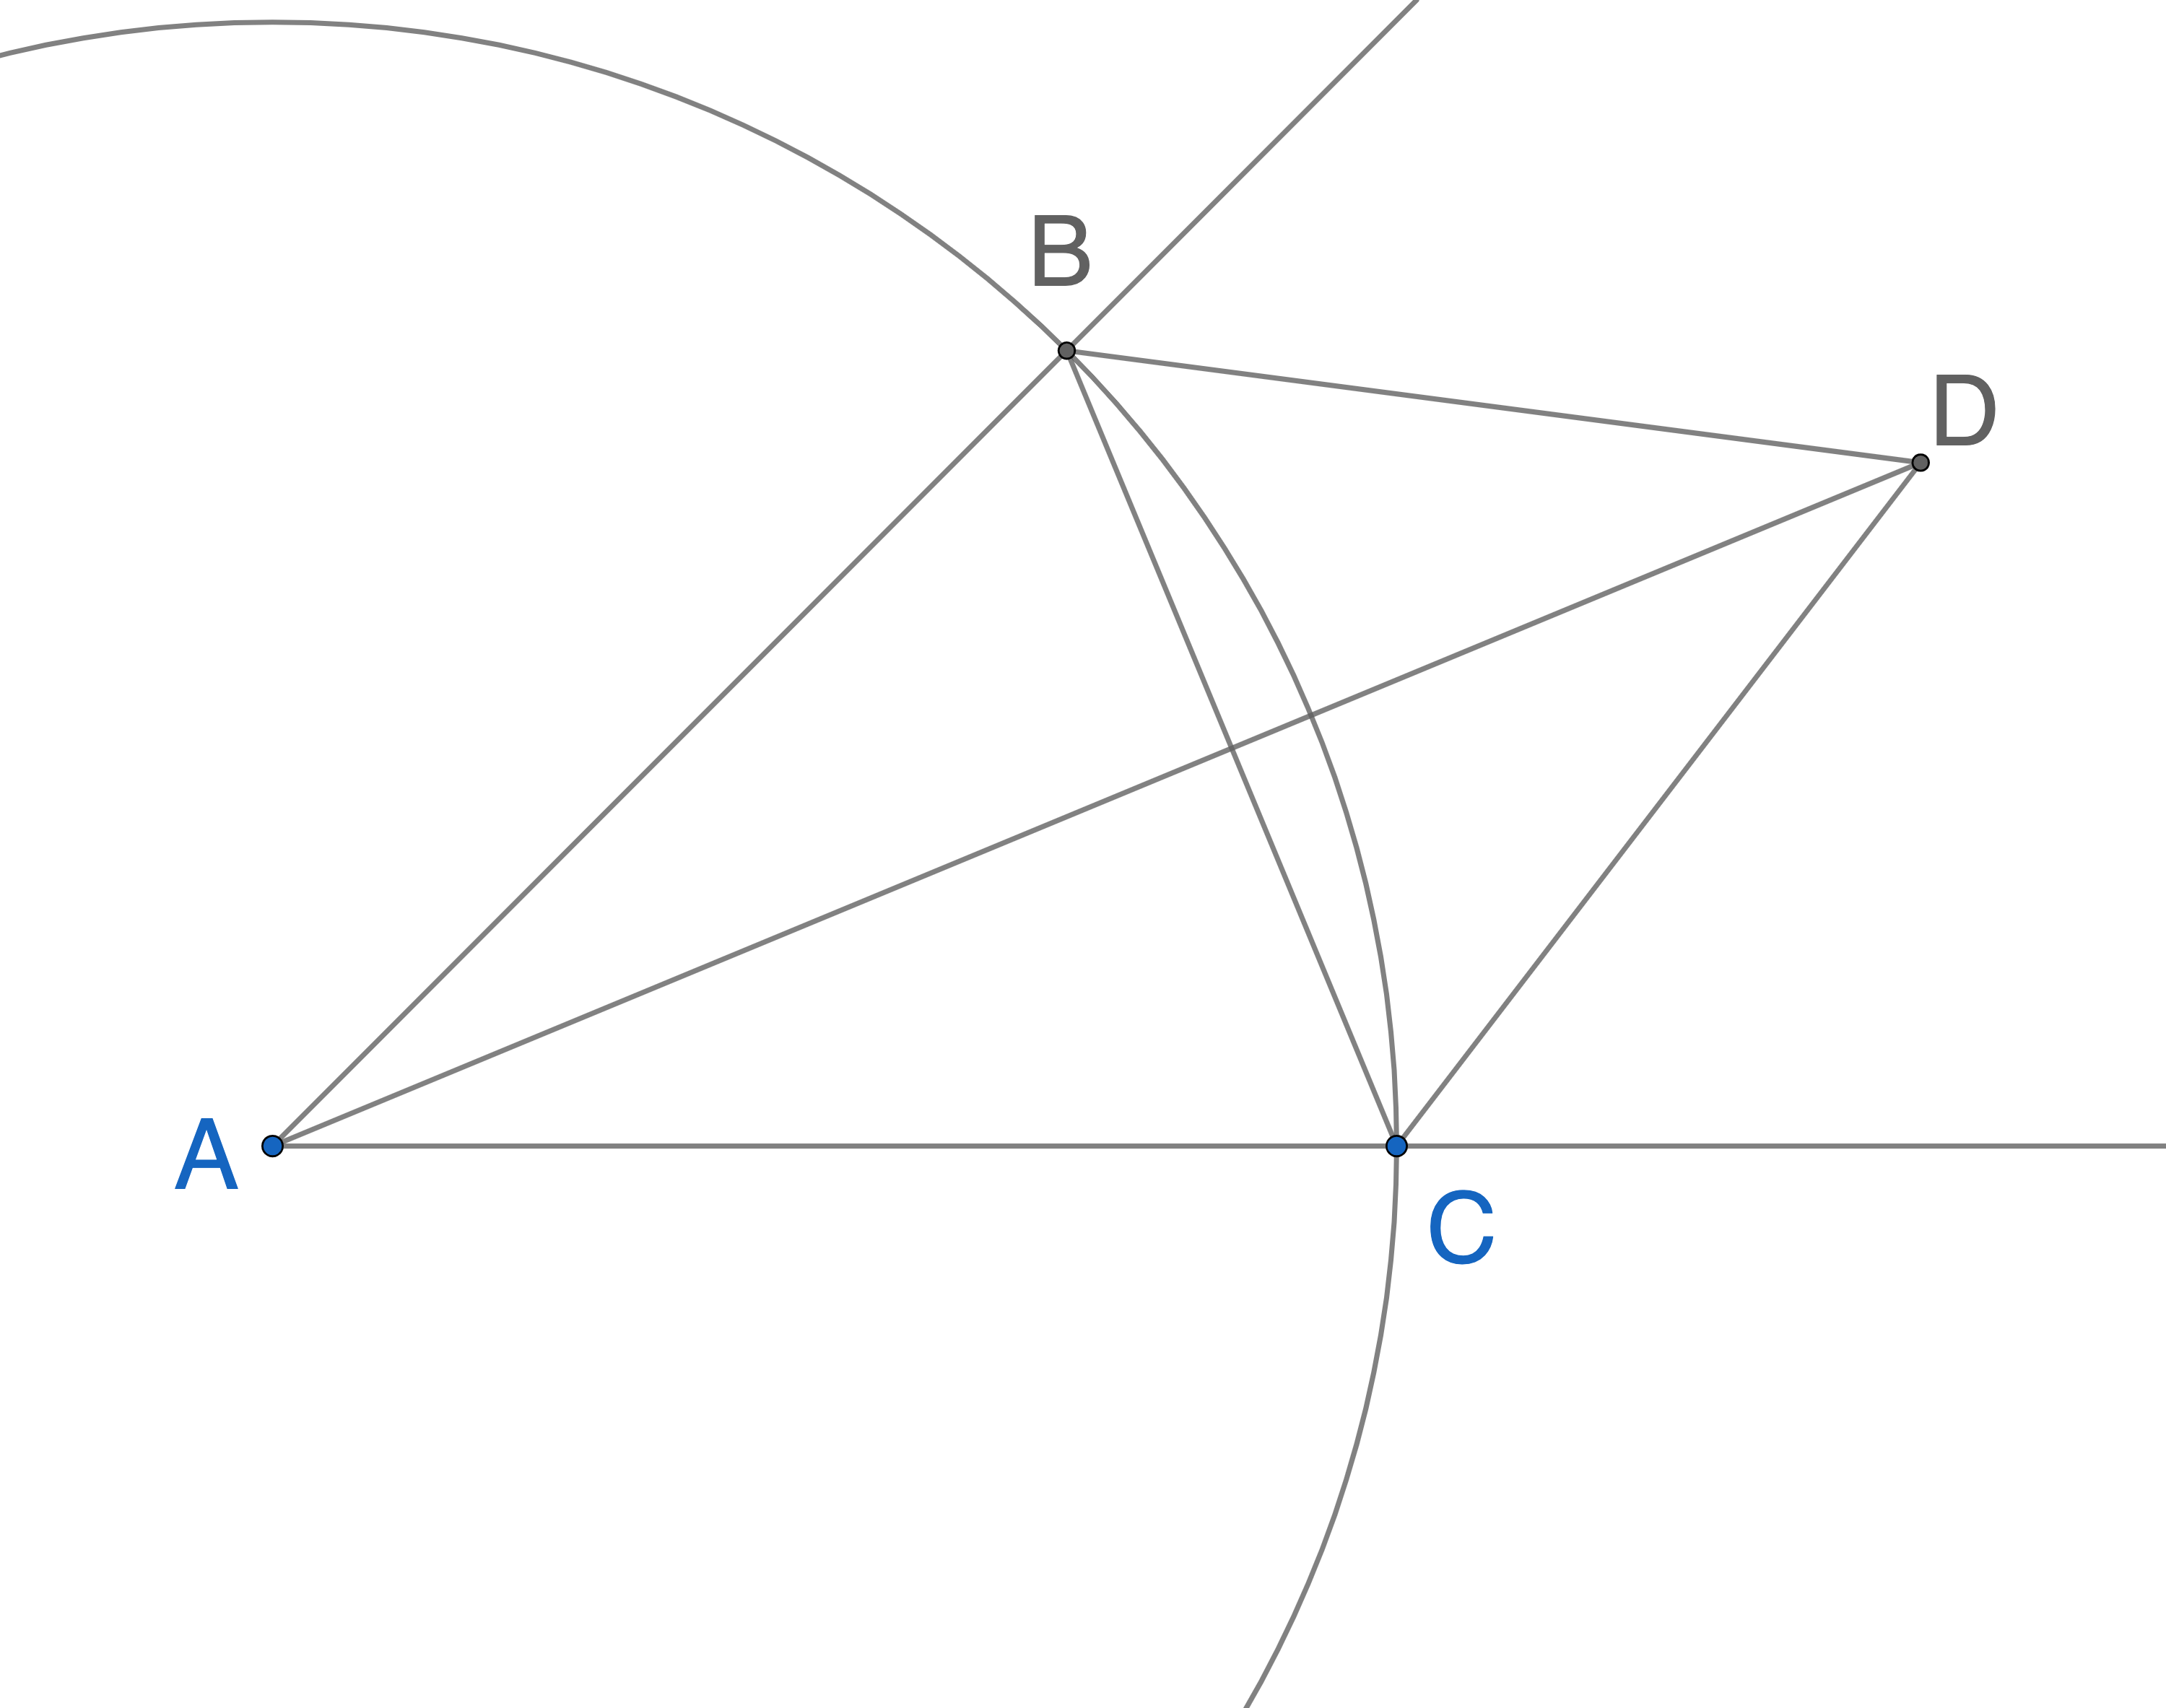
\includegraphics[width=0.35\textwidth]{angbisector}
\end{wrapfigure}
Given an angle formed by two rays extending from a point $A$, we draw a circle of arbitrary radius [Euclid Post.\@ 3] and label its points of intersection on the two rays $B$ and $C$. Now, with $\overline{\rm BC}$ as its base, we construct the equilateral triangle $\triangle{BCD}$, choosing point $D$ as the further one from A. We then consider $\triangle{ABD}$ and $\triangle{ACD}$. They share the side $\overline{\rm AD}$. We have that $\overline{\rm BD} \cong \overline{\rm CD}$ as they are both part of the same equilateral triangle. Finally, $\overline{\rm BC} \cong \overline{\rm AC}$ as they are radii of the same circle centered at $A$. By [1.3], $\triangle{ABD} \cong\triangle{ACD}$. From this we have $\angle BAD \cong \angle DAC$, meaning $\overline{\rm AD}$ bisects $\angle BAC$.
\section{Isosceles Angle Congruence}
\begin{wrapfigure}{r}{0.35\textwidth} %this figure is placed at the right
    \centering
    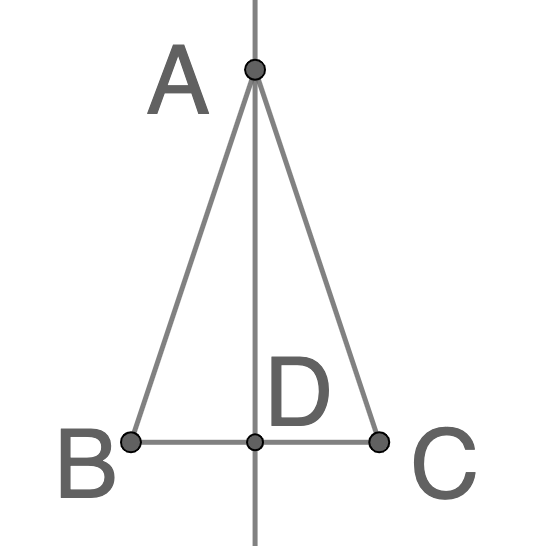
\includegraphics[width=0.25\textwidth]{ISOC}
\end{wrapfigure}
The angles opposite the congruent sides of an isosceles triangle are congruent.
\\[\baselineskip]
\textit{Proof.} Let $\triangle{ABC}$ be isosceles, and let $\overline{\rm AB} \cong \overline{\rm AC}$. Construct the angle bisector of $\angle a$ [1.2.3] and extend it to intersect with $\overline{\rm BC}$, labeling the point of intersection $D$. Consider $\triangle{ADC}$ and $\triangle{BDC}$. We know since $\overline{\rm AD}$ is the angle bisector of $\angle a$, so $\angle BAD \cong \angle CAD$. The triangles have $\overline{\rm AD}$ in common, and have $\overline{\rm AB} \cong \overline{\rm AC}$. By [1.1], $\triangle{ADC} \cong \triangle{BDC}$, giving that $\angle ABC \cong \angle ACB$.
\section{Isosceles Side Congruence}
\begin{wrapfigure}{r}{0.35\textwidth} %this figure is placed at the right
    \centering
    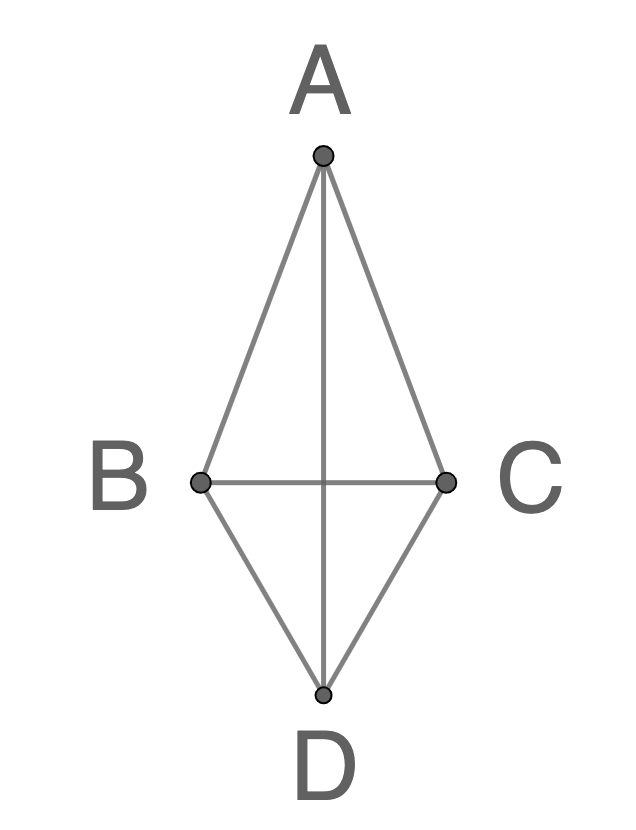
\includegraphics[width=0.25\textwidth]{ISOC2}
\end{wrapfigure}
If two angles of a triangle are congruent, the sides opposite those angles are congruent (and so the triangle is isosceles). Note that this is the converse of [1.3].
\\[\baselineskip]
\textit{Proof.} Let $\triangle{ABC}$ have $\angle b \cong \angle c$. With base $\overline{\rm BC}$ we construct the equilateral triangle $\triangle{BCD}$, choosing $D$ as the further point from $A$ (see the note to [1.2.1]). Draw the line segment $\overline{\rm AD}$.  Consider the triangles $\triangle{ABD}$ and $\triangle{ACD}$. These have $\overline{\rm AD}$ in common, have $\angle ADB \cong \angle ADC$ since they are the angles to an equilateral triangle, and have $\overline{\rm BD} \cong \overline{\rm DC}$, since these are the sides of an equilateral triangle. By [1.1] we have $\triangle{ABD} \cong \triangle{ACD}$, which gives $\overline{\rm AB} \cong \overline{\rm AC}$.
\section{Side-Side-Side Congruence}
\begin{wrapfigure}{r}{0.35\textwidth} %this figure is placed at the right
    \centering
    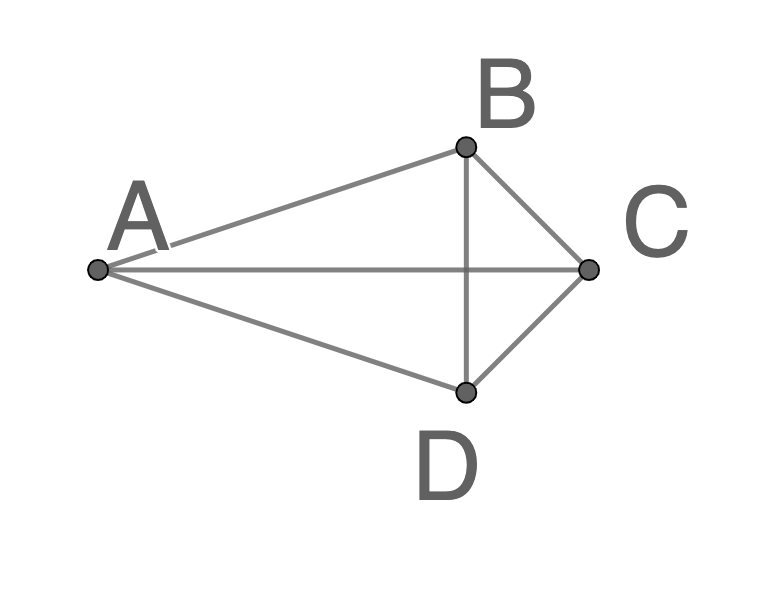
\includegraphics[width=0.35\textwidth]{SSS}
\end{wrapfigure}
Two triangles are congruent if the three sides of one are congruent respectively to the three sides of the other.
\\[\baselineskip]
\textit{Proof.} Let $\triangle{ABC}$ and $\triangle{A'C'D}$ have $|\overline{\rm AC}|=|\overline{\rm A'C'}|$, $|\overline{\rm AB}|=|\overline{\rm A'D}|$, and $|\overline{\rm BC}|=|\overline{\rm DC'}|$. Move $\triangle{A'C'D}$ so that $\overline{\rm A'C'}$ coincides with $\overline{\rm AC}$, and so that $B$ and $D$ are on different sides of $\overline{\rm AC}$. Draw $\overline{\rm BD}$. Now, $\triangle{ABD}$ is isosceles, and so $|\angle ABD| = |\angle ADB|$. $\triangle{CBD}$ is also isosceles, and so $|\angle CBD| = |\angle CDB|$. Since $|\angle ABC| = |\angle ABD|+|\angle CBD|$, and $|\angle ADC| = |\angle ADB|+|\angle CDB|$, substituting our previous angle equalities gives $\angle ABC \cong \angle ADC$. Then we have $\triangle{ABC} \cong \triangle{A'C'D}$ by [1.1].

\subsubsection{Equilateral triangles have equal angles}
\textit{Proof.} This is a corollary of [1.5], but it is worth noting as it will be used later.

\subsection{Construction of a Perpendicular Line off a Given Point}
\begin{wrapfigure}{r}{0.35\textwidth} %this figure is placed at the right
    \centering
    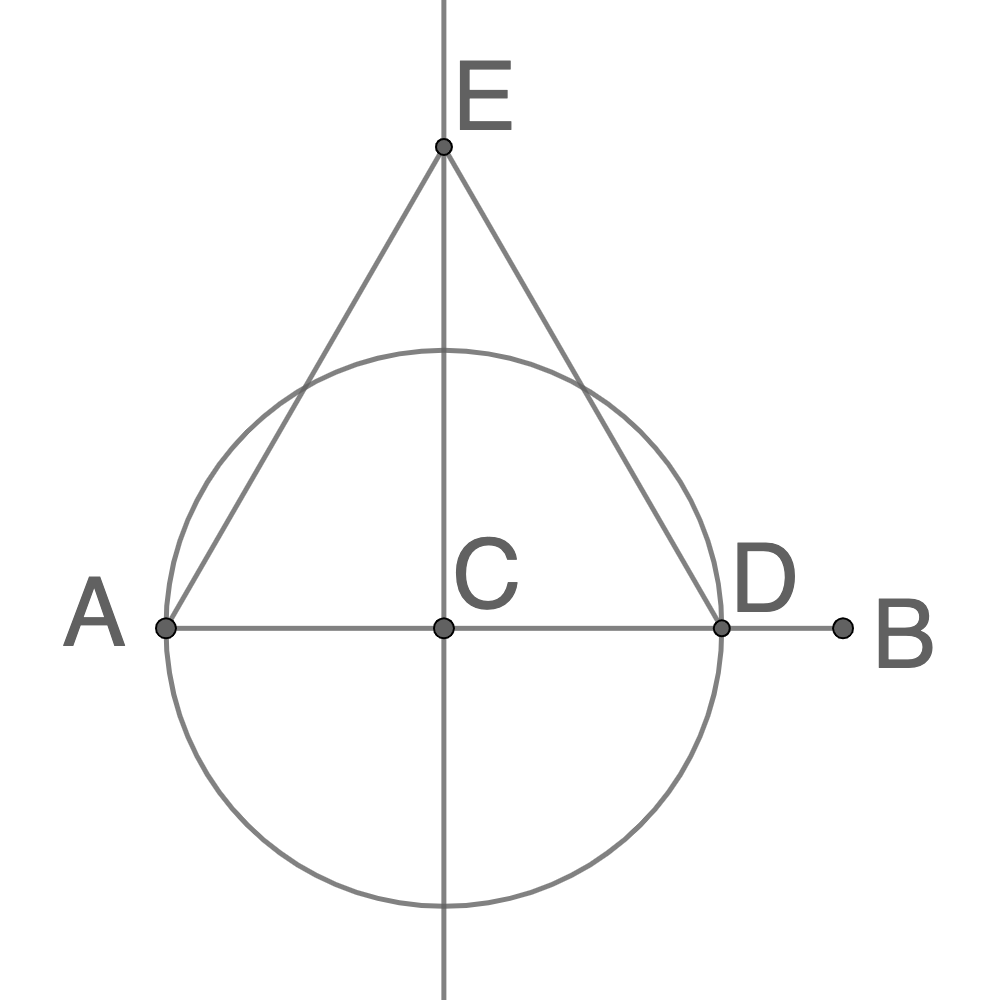
\includegraphics[width=0.25\textwidth]{perp}
\end{wrapfigure}
Given a line segment $\overline{\rm AB}$, and a point $C$ on $\overline{\rm AB}$, we will construct a line extending from $C$ that is perpendicular to $\overline{\rm AB}$ (makes right angles with $\overline{\rm AB}$).
\\[\baselineskip]
Centered at $C$, draw the circle $\alpha$ with the smaller of $|\overline{\rm AC}|$, $|\overline{\rm CB}|$ as its radius. WLOG, we will assume it is of radius $|\overline{\rm AC}|$. Let $D$ be the point of intersection of $\alpha$ with $|\overline{\rm AB}|$ that is not $A$. Then, draw an equilateral triangle $\triangle{ADE}$ with base $|\overline{\rm AD}|$. Construct the line $|\overrightarrow{\rm EC}|$. We claim that $|\overrightarrow{\rm EC}|$ is perpendicular to $\overline{\rm AB}$.
\\Clearly $\angle ACE$ and $\angle DCE$ are supplementary, and [1.5] shows that $\triangle{ACE}$ and $\triangle{DCE}$ are congruent. Since $\angle ACE$ and $\angle DCE$ are supplementary angles congruent to each other, they are right by definition.
\\[\baselineskip]
\section{Supplementary Angle Congruence}
\begin{wrapfigure}{r}{0.35\textwidth} %this figure is placed at the right
    \centering
    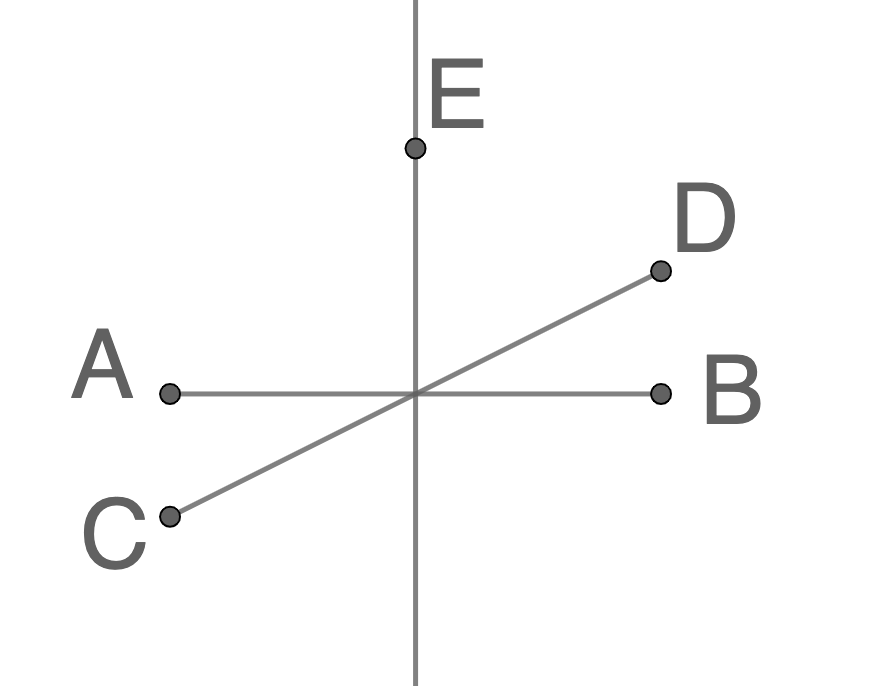
\includegraphics[width=0.25\textwidth]{supp}
\end{wrapfigure}
Supplementary angles are congruent to two right angles. Recall that supplementary angles are the angles formed by the intersection of two lines which share a common line segment.
\\[\baselineskip]
\textit{Proof.} Consider the supplementary angles $\angle AFD$ and $\angle DFB$ formed by the intersection of $\overline{\rm AB}$ with $\overline{\rm CD}$, labeling their point of intersection $F$. From $F$ construct a line perpendicular to $\overline{\rm AB}$ [1.5.1]. Label a point on this line $E$. If $\angle AFD \cong \angle AFE$, the proof is trivial, so we will assume that $\overline{\rm FE}$ and $\overline{\rm FD}$ do not coincide, WLOG having $\angle AFE$ within $\angle AFD$.
\\Then, $\angle AFD = \angle AFE + \angle EFD$, and $\angle EFB = \angle EFD + \angle DFB$. Adding these equalities gives: \begin{displaymath}
\angle AFD + \angle EFD + \angle DFB = \angle AFE + \angle EFD + \angle EFB
\end{displaymath}
Which may simplify to\begin{displaymath}
\angle AFD +\angle DFB = \angle AFE + \angle EFB
\end{displaymath}
Which is exactly our theorem, as  $\angle AFE + \angle EFB$ are two right angles.

\section{Vertical Angle Congruence}
Vertical angles are congruent. Recall that vertical angles (also called opposite angles) are the angles formed by the intersection of two lines which do not share a common line segment.
\\
\begin{wrapfigure}{r}{0.35\textwidth} %this figure is placed at the right
    \centering
    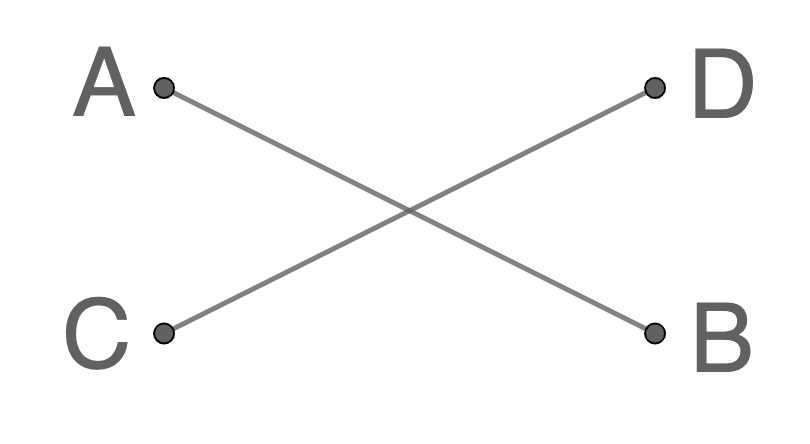
\includegraphics[width=0.25\textwidth]{vert}
\end{wrapfigure}
\\[\baselineskip]
\textit{Proof.} Consider the vertical angles $\angle AEC$ and $\angle DEB$ formed by the intersection of $\overline{\rm AB}$ with $\overline{\rm CD}$, labeling their point of intersection $E$. Let $\alpha$ represent the measure of two right angles. By [1.6], we have $\angle AEC + \angle AED = \alpha$, and by [1.6] we have $\angle DEB + \angle AED = \alpha$. From this we have $\angle AEC + \angle AED = \angle DEB + \angle AED$, and applying the cancellation property gives $\angle AEC = \angle DEB$.



\end{document}
